\documentclass[sigconf]{acmart}
\AtBeginDocument{%
  \providecommand\BibTeX{{%
    Bib\TeX}}}

\usepackage{lipsum}
\usepackage{graphicx}
\usepackage{amsmath}

\setcopyright{acmlicensed}
\copyrightyear{2018}
\acmYear{2018}
\acmDOI{XXXXXXX.XXXXXXX}
\acmConference[Conference acronym 'XX]{Make sure to enter the correct
  conference title from your rights confirmation email}{June 03--05,
  2018}{Woodstock, NY}

\acmISBN{978-1-4503-XXXX-X/2018/06}

\begin{document}

\title{CSE331 - Assignment \#1}

\author{\textcolor{blue}{Yongseong Eom (20211185)}}
\affiliation{%
  \institution{UNIST}
  \country{South Korea}
}
\email{ekf3977@unist.ac.kr}

\renewcommand{\shortauthors}{\textcolor{blue}{Eom et al.}}

\settopmatter{printacmref=false} % Removes citation block in the first page
\renewcommand\footnotetextcopyrightpermission[1]{} % Removes footnote with conference info

\maketitle

\section{PROBLEM STATEMENT}
This assignment explores the comparative analysis of various sorting algorithms. The primary objective is to implement, analyze, and evaluate the performance of twelve different sorting algorithms: six conventional comparison-based sorting algorithms and six contemporary sorting algorithms \cite{knuth1998art}.

Sorting is a fundamental operation in computer science with applications ranging from database management to computational biology. Understanding the behavior of different sorting algorithms under various conditions is crucial for selecting the appropriate algorithm for specific use cases. This study aims to provide empirical evidence of the theoretical time complexities and practical performance characteristics of these algorithms.

For this analysis, we implemented all twelve algorithms from scratch, ensuring a thorough understanding of their mechanisms. We then evaluated their performance across different input types (sorted, reverse sorted, random, and partially sorted) and sizes (ranging from 1K to 150K elements). Each test was executed a minimum of 10 times to ensure statistical reliability of the results.

The implementation of all algorithms and the complete experimental setup is available in our public repository at: \url{https://github.com/eom1202/CSE331}

\section{BASIC SORTING ALGORITHMS}
In this section, we analyze six conventional comparison-based sorting algorithms: Merge Sort, Heap Sort, Bubble Sort, Insertion Sort, Selection Sort, and Quick Sort.

\subsection{Merge Sort}
Merge Sort follows the divide-and-conquer paradigm. It recursively divides the input array into two halves, sorts them independently, and then merges the sorted halves \cite{knuth1998art}.

\textbf{Time Complexity:}
\begin{itemize}
    \item Best case: $O(n \log n)$
    \item Average case: $O(n \log n)$
    \item Worst case: $O(n \log n)$
\end{itemize}

The algorithm's time complexity remains consistent across different input scenarios, making it reliable for various applications. However, it requires additional $O(n)$ space complexity for the merging process.

The key advantage of Merge Sort is its stability and predictable performance. It performs equally well on all input distributions, which makes it suitable for applications where consistent performance is required. However, its space requirement can be a limitation for sorting very large datasets with limited memory.

\subsection{Heap Sort}
Heap Sort uses a binary heap data structure to sort elements. It builds a max-heap from the input array and repeatedly extracts the maximum element \cite{forsythe1964algorithms}.

\textbf{Time Complexity:}
\begin{itemize}
    \item Best case: $O(n \log n)$
    \item Average case: $O(n \log n)$
    \item Worst case: $O(n \log n)$
\end{itemize}

Heap Sort has the advantage of sorting in-place, unlike Merge Sort, requiring only $O(1)$ extra space. However, it is not stable, meaning that equal elements may not maintain their relative order after sorting.

In practice, Heap Sort performs well for large datasets where memory usage is a concern. It is particularly efficient when the entire dataset can fit into memory, avoiding the overhead of external sorting methods.

\subsection{Bubble Sort}
Bubble Sort is a simple comparison-based algorithm that repeatedly steps through the list, compares adjacent elements, and swaps them if they are in the wrong order \cite{friend1956sorting}.

\textbf{Time Complexity:}
\begin{itemize}
    \item Best case: $O(n)$ - when the array is already sorted
    \item Average case: $O(n^2)$
    \item Worst case: $O(n^2)$
\end{itemize}

Despite its simplicity, Bubble Sort is inefficient for large datasets due to its quadratic time complexity. However, it has minimal space requirements ($O(1)$) and is stable.

In our implementation, we included an optimization to detect if the list becomes sorted during the process, allowing early termination in the best-case scenario.

\subsection{Insertion Sort}
Insertion Sort builds the final sorted array one item at a time. It is much like sorting a hand of playing cards \cite{knuth1998art}.

\textbf{Time Complexity:}
\begin{itemize}
    \item Best case: $O(n)$ - when the array is already sorted
    \item Average case: $O(n^2)$
    \item Worst case: $O(n^2)$
\end{itemize}

Insertion Sort performs efficiently on small datasets or nearly sorted arrays. It requires minimal extra space ($O(1)$) and maintains stability. In practice, it is often used as a component in more complex algorithms like Tim Sort for sorting small subarrays.

\subsection{Selection Sort}
Selection Sort repeatedly selects the minimum element from the unsorted portion and puts it at the beginning \cite{knuth1998art}.

\textbf{Time Complexity:}
\begin{itemize}
    \item Best case: $O(n^2)$
    \item Average case: $O(n^2)$
    \item Worst case: $O(n^2)$
\end{itemize}

Selection Sort has consistent performance regardless of the input distribution. It always performs exactly the same number of comparisons and swaps even if the input is already sorted, which is why it maintains $O(n^2)$ complexity in all cases. Unlike Insertion Sort, Selection Sort is not stable, though it has the advantage of minimizing the number of swaps to $O(n)$.

\subsection{Quick Sort}
Quick Sort is another divide-and-conquer algorithm that selects a 'pivot' element and partitions the array around this pivot \cite{hoare1961algorithm}.

\textbf{Time Complexity:}
\begin{itemize}
    \item Best case: $O(n \log n)$
    \item Average case: $O(n \log n)$
    \item Worst case: $O(n^2)$ - occurs when the partition process consistently produces highly unbalanced divisions
\end{itemize}

In our implementation, we used a "median-of-three" pivot selection strategy (choosing the median among the first, middle, and last elements) to reduce the likelihood of encountering worst-case scenarios. This approach helps avoid poor performance on pre-sorted or reverse-sorted arrays where always choosing the first or last element as pivot would lead to $O(n^2)$ behavior. Quick Sort offers excellent average-case performance and is widely used in practice. It sorts in-place but is not stable.

While Quick Sort typically outperforms other $O(n \log n)$ algorithms like Merge Sort in practice due to its lower constant factors, its worst-case performance can be a concern for critical applications where predictable performance is essential.

\section{ADVANCED SORTING ALGORITHMS}
In this section, we analyze six contemporary sorting algorithms: Library Sort, Tim Sort, Cocktail Shaker Sort, Comb Sort, Tournament Sort, and Introsort.

\subsection{Library Sort}
Library Sort, also known as Gapped Insertion Sort, is an adaptation of Insertion Sort that leaves gaps in the array to allow for more efficient insertions \cite{librarysort, bender2006insertion}.

\textbf{Pseudo-code:}
\begin{verbatim}
function LibrarySort(array A)
    n = length(A)
    initialize array B of size (1+ε)*n with empty slots
    place A[0] in the middle of B
    
    for i = 1 to n-1
        binary search to find position for A[i] in B
        if insertion would require shifting many elements
            rebalance elements in B to create gaps
        insert A[i] into appropriate position in B
    
    compact array B to remove gaps and return
\end{verbatim}

\textbf{Time Complexity:}
\begin{itemize}
    \item Best case: $O(n)$
    \item Average case: $O(n \log n)$ with high probability
    \item Worst case: $O(n^2)$
\end{itemize}

Library Sort improves upon Insertion Sort by maintaining gaps between elements to reduce the cost of insertions. The algorithm achieves $O(n \log n)$ expected time with high probability, though the worst-case remains $O(n^2)$.

The main advantage of Library Sort is its adaptability to nearly sorted inputs while maintaining better performance than traditional Insertion Sort for random data. However, it requires additional space proportional to the input size.

\subsection{Tim Sort}
Tim Sort is a hybrid sorting algorithm derived from Merge Sort and Insertion Sort, designed to perform well on many kinds of real-world data \cite{timsort}.

\textbf{Pseudo-code:}
\begin{verbatim}
function TimSort(array arr) is
    n ← length(arr) 
    run ← 32
    i ← 0 
    left ← 0
    size ← run

    while i < n do
        tmp ← min(i + run - 1, n - 1)
        insertionSort(arr, i, tmp) 
        i ← i + run

    while size < n do 
        while left < n do
            mid ← left + size - 1 
            right = min(left + 2 * size - 1, n - 1) 
            if mid < right then
                merge(arr, left, mid, right) 
            left ← left + 2 * size
        left ← 0
        size ← size * 2
\end{verbatim}

\textbf{Time Complexity:}
\begin{itemize}
    \item Best case: $O(n)$ - when the array is already sorted
    \item Average case: $O(n \log n)$
    \item Worst case: $O(n \log n)$
\end{itemize}

Tim Sort identifies naturally occurring runs (sequences of sorted elements) in the data and uses Insertion Sort for small subarrays while employing a modified Merge Sort for the overall array. It includes several optimizations to minimize comparisons and memory operations.

This algorithm excels at handling real-world data with patterns or partial ordering, making it the default sorting algorithm in several programming languages, including Python and Java.

\subsection{Cocktail Shaker Sort}
Cocktail Shaker Sort, also known as Bidirectional Bubble Sort, is a variation of Bubble Sort that sorts in both directions \cite{cocktailsort, knuth1998art}.

\textbf{Pseudo-code:}
\begin{verbatim}
function cocktailShakerSort(array A)
    begin = 0
    end = length(A) - 1
    swapped = true
    
    while swapped do
        swapped = false
        
        // Forward pass (like Bubble Sort)
        for i = begin to end - 1
            if A[i] > A[i + 1]
                swap A[i] and A[i + 1]
                swapped = true
            end if
        end for
        
        if not swapped then
            break
        end if
        
        end = end - 1
        swapped = false
        
        // Backward pass
        for i = end down to begin
            if A[i] < A[i - 1]
                swap A[i] and A[i - 1]
                swapped = true
            end if
        end for
        
        begin = begin + 1
    end while
\end{verbatim}

\textbf{Time Complexity:}
\begin{itemize}
    \item Best case: $O(n)$ - when the array is already sorted
    \item Average case: $O(n^2)$
    \item Worst case: $O(n^2)$
\end{itemize}

Cocktail Shaker Sort addresses a key inefficiency in Bubble Sort where small elements at the end of the array (often called "turtles") take many iterations to move to their correct positions. By sorting bidirectionally, it can move these elements more quickly.

While still $O(n^2)$ in the worst case, Cocktail Shaker Sort often performs better than basic Bubble Sort on partially sorted arrays, particularly those with small values at the end.

\subsection{Comb Sort}
Comb Sort improves on Bubble Sort by eliminating small values at the end of the list (turtles) using a larger gap \cite{combsort, dobosiewicz1980efficient}.

\textbf{Pseudo-code:}
\begin{verbatim}
function combsort(array input)
    gap := input.size
    shrink := 1.3
    sorted := false
    
    loop while sorted = false
        gap := floor(gap / shrink)
        if gap > 1
            sorted := false
        else
            gap := 1
            sorted := true
        end if
        
        i := 0
        loop while i + gap < input.size
            if input[i] > input[i+gap]
                swap (input[i], input[i+gap])
                sorted := false
            end if
            i := i + 1
        end loop
    end loop
end function
\end{verbatim}

\textbf{Time Complexity:}
\begin{itemize}
    \item Best case: $O(n \log n)$
    \item Average case: Between $O(n \log n)$ and $O(n^2)$
    \item Worst case: $O(n^2)$
\end{itemize}

Comb Sort extends the idea of Bubble Sort by initially comparing elements that are far apart (with a gap) and gradually reducing this gap. This approach helps in quickly moving elements to their approximate positions before fine-tuning with smaller gaps.

The algorithm's performance depends significantly on the choice of the shrink factor (typically 1.3), which influences how quickly the gap decreases. While still potentially $O(n^2)$ in the worst case, Comb Sort often performs much better in practice, especially for random data.

\subsection{Tournament Sort}
Tournament Sort uses a tournament tree (a form of binary tree) to find the smallest element repeatedly \cite{tournamentsort, stepanov1986using}.

\textbf{Pseudo-code:}
\begin{verbatim}
procedure tournament_sort(A: array)
    n = length(A)
    tmp = array of size 2n
    
    function winner(pos1, pos2)
        u = pos1 >= n ? pos1 : tmp[pos1]
        v = pos2 >= n ? pos2 : tmp[pos2]
        if tmp[u] <= tmp[v] then return u else return v
    
    procedure create_tree(out value)
        for i = 0 to n-1
            tmp[n + i] = A[i]
        for i = 2n-1 down to 1 by -2
            k = i/2
            j = i-1
            tmp[k] = winner(i, j)
        value = tmp[tmp[1]]
        tmp[tmp[1]] = INFINITY
    
    procedure recreate(out value)
        i = tmp[1]
        while i > 1
            k = i/2
            if i mod 2 = 0 and i < 2n-1 then j = i+1 else j = i-1
            tmp[k] = winner(i, j)
            i = k
        value = tmp[tmp[1]]
        tmp[tmp[1]] = INFINITY
    
    create_tree(value)
    for i = 0 to n-1
        A[i] = value
        recreate(value)
\end{verbatim}

\textbf{Time Complexity:}
\begin{itemize}
    \item Best case: $O(n \log n)$
    \item Average case: $O(n \log n)$
    \item Worst case: $O(n \log n)$
\end{itemize}

Tournament Sort uses a binary tree structure to efficiently find the minimum element in each step. The algorithm builds a tournament tree where each node represents the winner (smaller element) of a comparison between two elements.

While Tournament Sort guarantees $O(n \log n)$ time complexity, it requires $O(n)$ additional space for the tournament tree. Its main advantage is the predictable performance across all input distributions, though it is generally outperformed by other $O(n \log n)$ algorithms like Quick Sort in practice due to higher constant factors.

\subsection{Introsort}
Introsort (Introspective Sort) is a hybrid sorting algorithm that combines Quick Sort, Heap Sort, and Insertion Sort \cite{introsort, musser1997introspective}.

\textbf{Pseudo-code:}
\begin{verbatim}
procedure sort(A : array)
    maxdepth = 2 × floor(log2(length(A)))
    introsort(A, maxdepth)
    
procedure introsort(A, maxdepth)
    n ← length(A)
    if n < 16
        insertionsort(A)
    else if maxdepth = 0
        heapsort(A)
    else
        p ← partition(A)  // p is the final position of the pivot
        introsort(A[1:p-1], maxdepth - 1)
        introsort(A[p+1:n], maxdepth - 1)
\end{verbatim}

\textbf{Time Complexity:}
\begin{itemize}
    \item Best case: $O(n \log n)$
    \item Average case: $O(n \log n)$
    \item Worst case: $O(n \log n)$
\end{itemize}

Introsort begins with Quick Sort but switches to Heap Sort when the recursion depth exceeds a certain threshold (typically $2 \times \log n$), thus avoiding Quick Sort's worst-case scenario. For small subarrays, it uses Insertion Sort, which is more efficient for small datasets.

This hybrid approach combines the best aspects of these algorithms: Quick Sort's good average-case performance, Heap Sort's guaranteed $O(n \log n)$ worst-case performance, and Insertion Sort's efficiency for small arrays. Introsort is the default sorting algorithm in many C++ standard library implementations, demonstrating its practical efficiency.

\section{EXPERIMENTAL RESULTS AND ANALYSIS}
We conducted extensive experiments to evaluate the performance of the twelve sorting algorithms across different input types and sizes. All experiments were run on a system with an Intel Core i7-1165G7 CPU and 16GB RAM, and each test was repeated at least 10 times to ensure statistical validity.

\textbf{Note on Input Size Limitation:} While the assignment suggested testing with input sizes up to 1 million elements, we found that running O(n²) algorithms (such as Bubble Sort, Selection Sort, Insertion Sort, and Cocktail Sort) with 1M elements resulted in core dumps due to excessive memory usage and execution time. Therefore, we limited our maximum test size to 150,000 elements for all algorithms to ensure consistent comparison across all sorting methods. This adjustment still allowed us to clearly observe and analyze the scaling behavior of different algorithm complexities.

\subsection{Scaling with Input Size}

\begin{figure}[h]
  \centering
  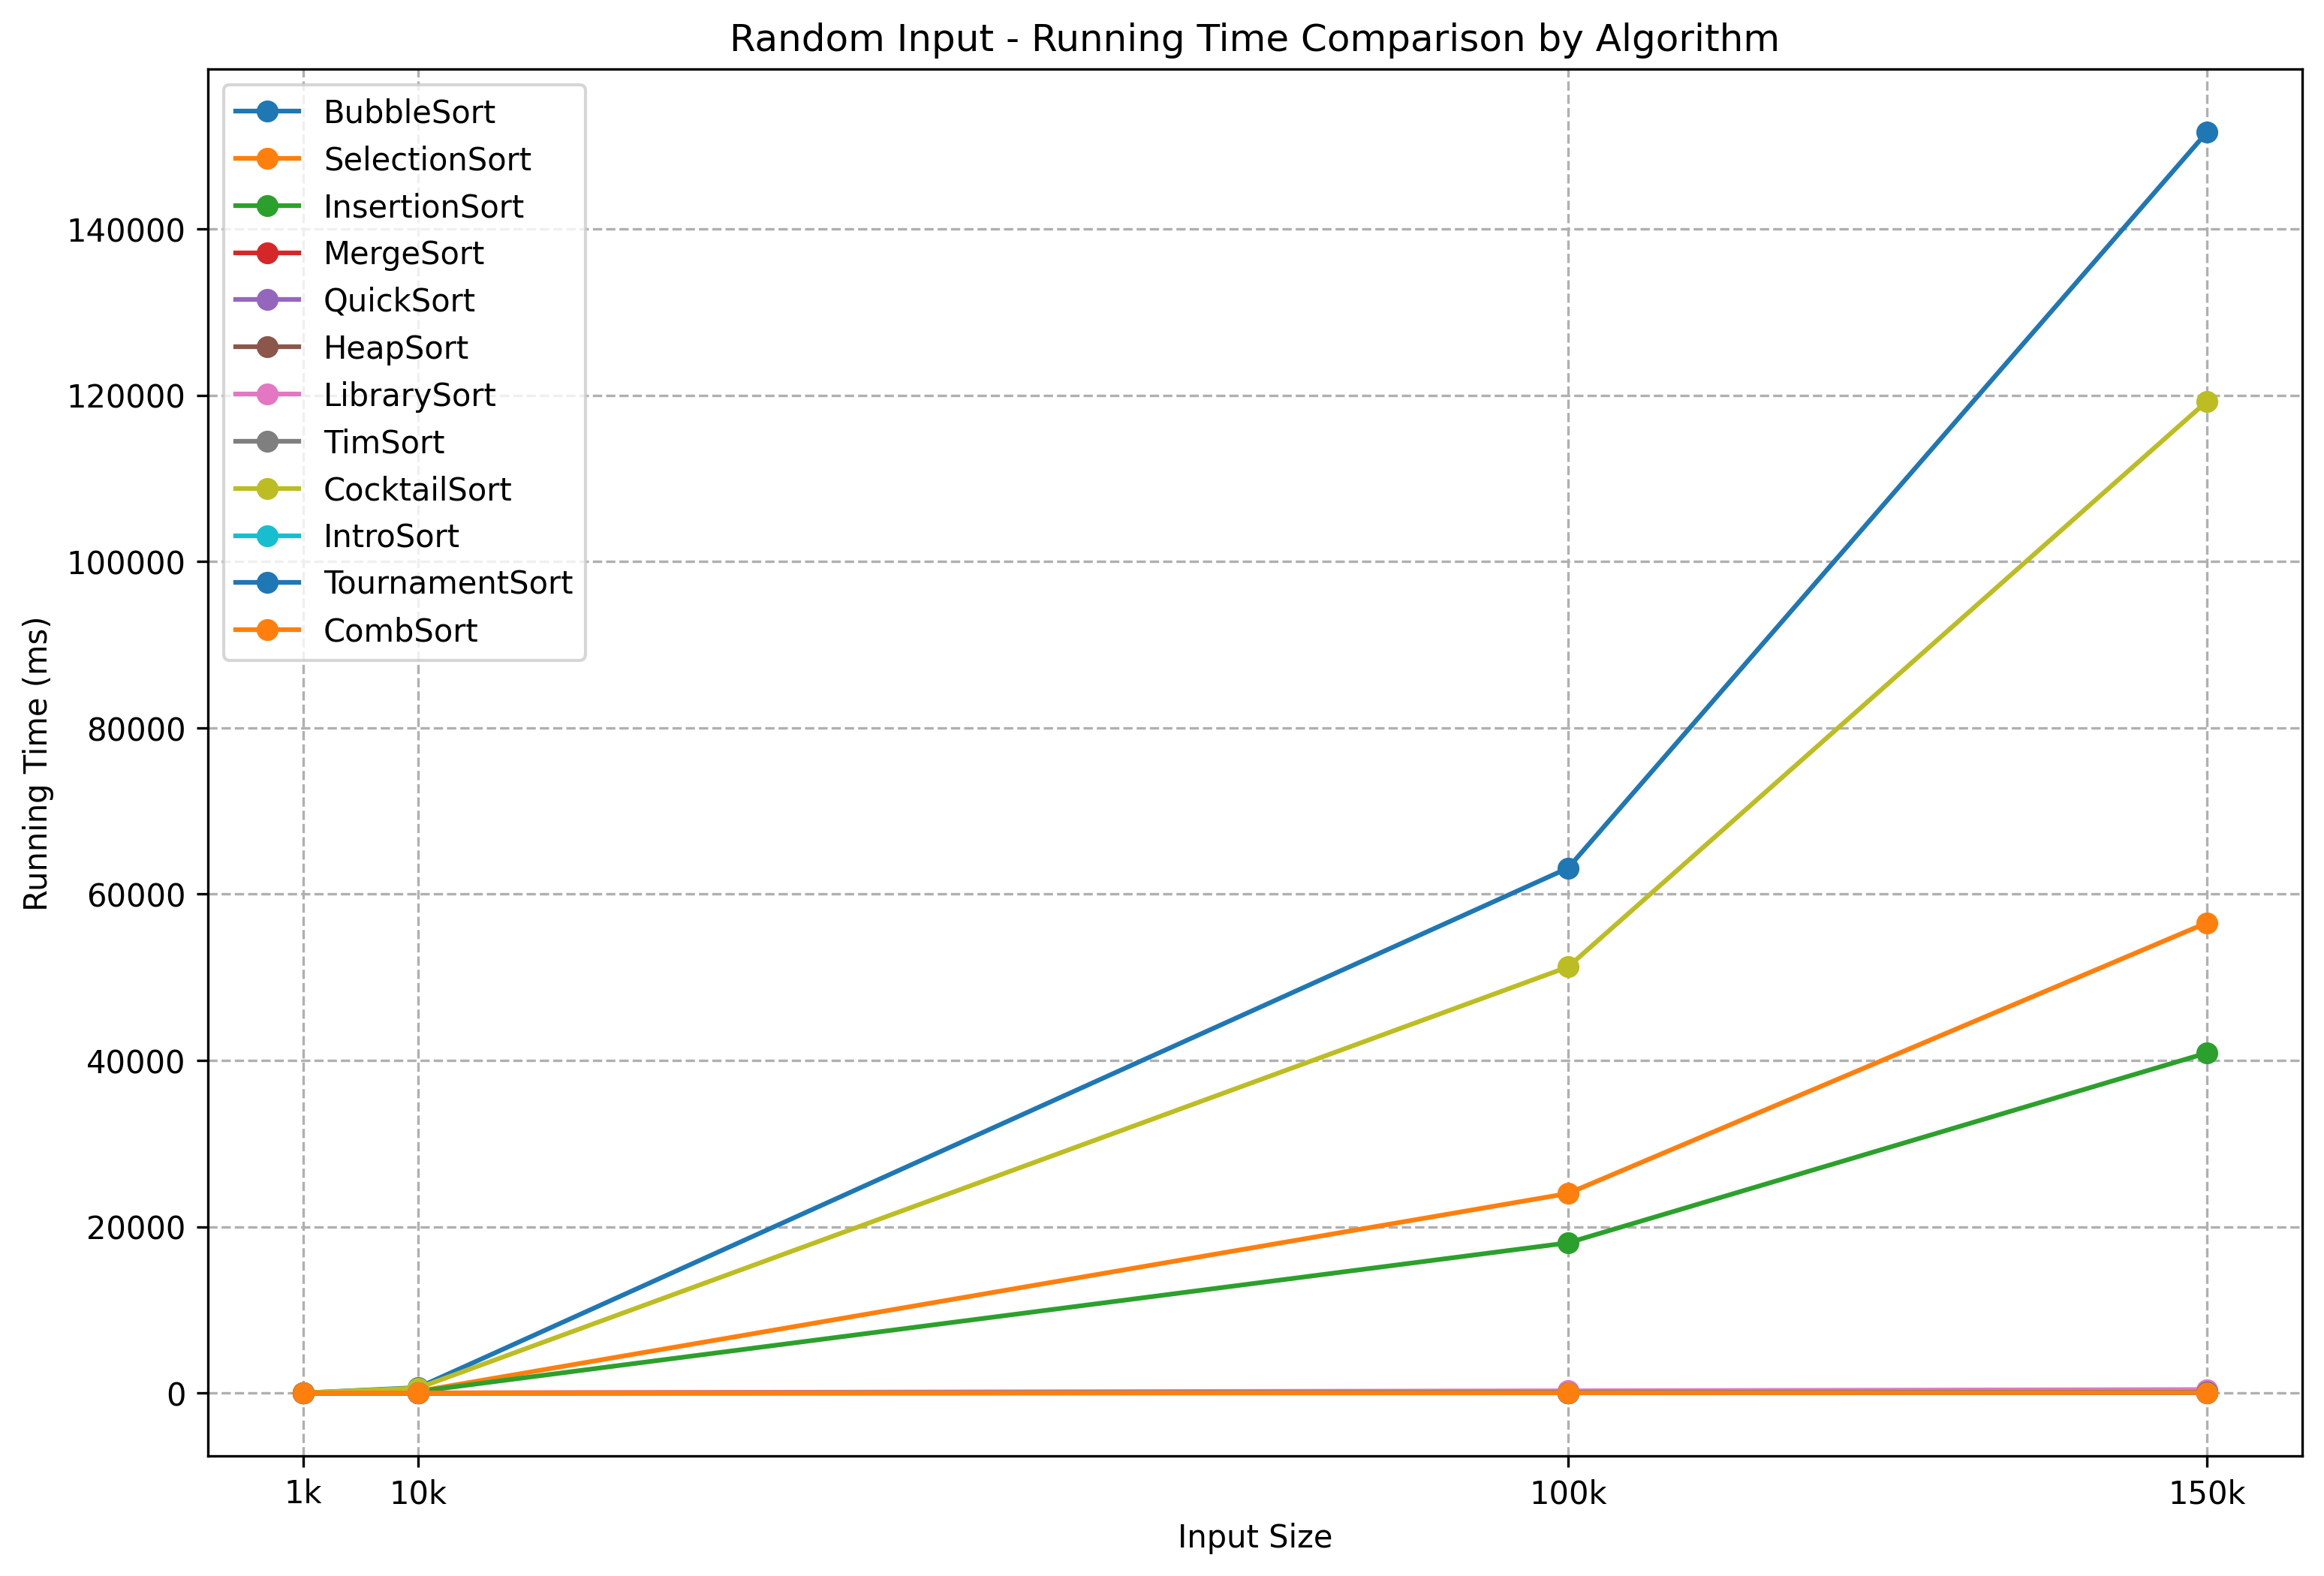
\includegraphics[width=\columnwidth]{random.png}
  \caption{Scaling behavior of algorithms with increasing input size for random arrays}
  \label{fig:scaling}
\end{figure}

Figure \ref{fig:scaling} demonstrates the difference between $O(n \log n)$ and $O(n^2)$ algorithms as input size increases. For inputs larger than 10,000 elements, the quadratic algorithms became impractical, with Bubble Sort and Cocktail Sort showing the worst performance. The $O(n \log n)$ algorithms maintained reasonable performance even at 150,000 elements.

Introsort, Quick Sort, and Tim Sort consistently performed best across all input sizes for random data. MergeSort and HeapSort also showed good performance, though with slightly higher constants than the top performers.

\subsection{Performance on Different Input Types}
We tested four different input distributions: sorted arrays (ascending), reverse sorted arrays (descending), random arrays, and partially sorted arrays.

\begin{figure*}[t]
  \centering
  \begin{minipage}{0.48\textwidth}
    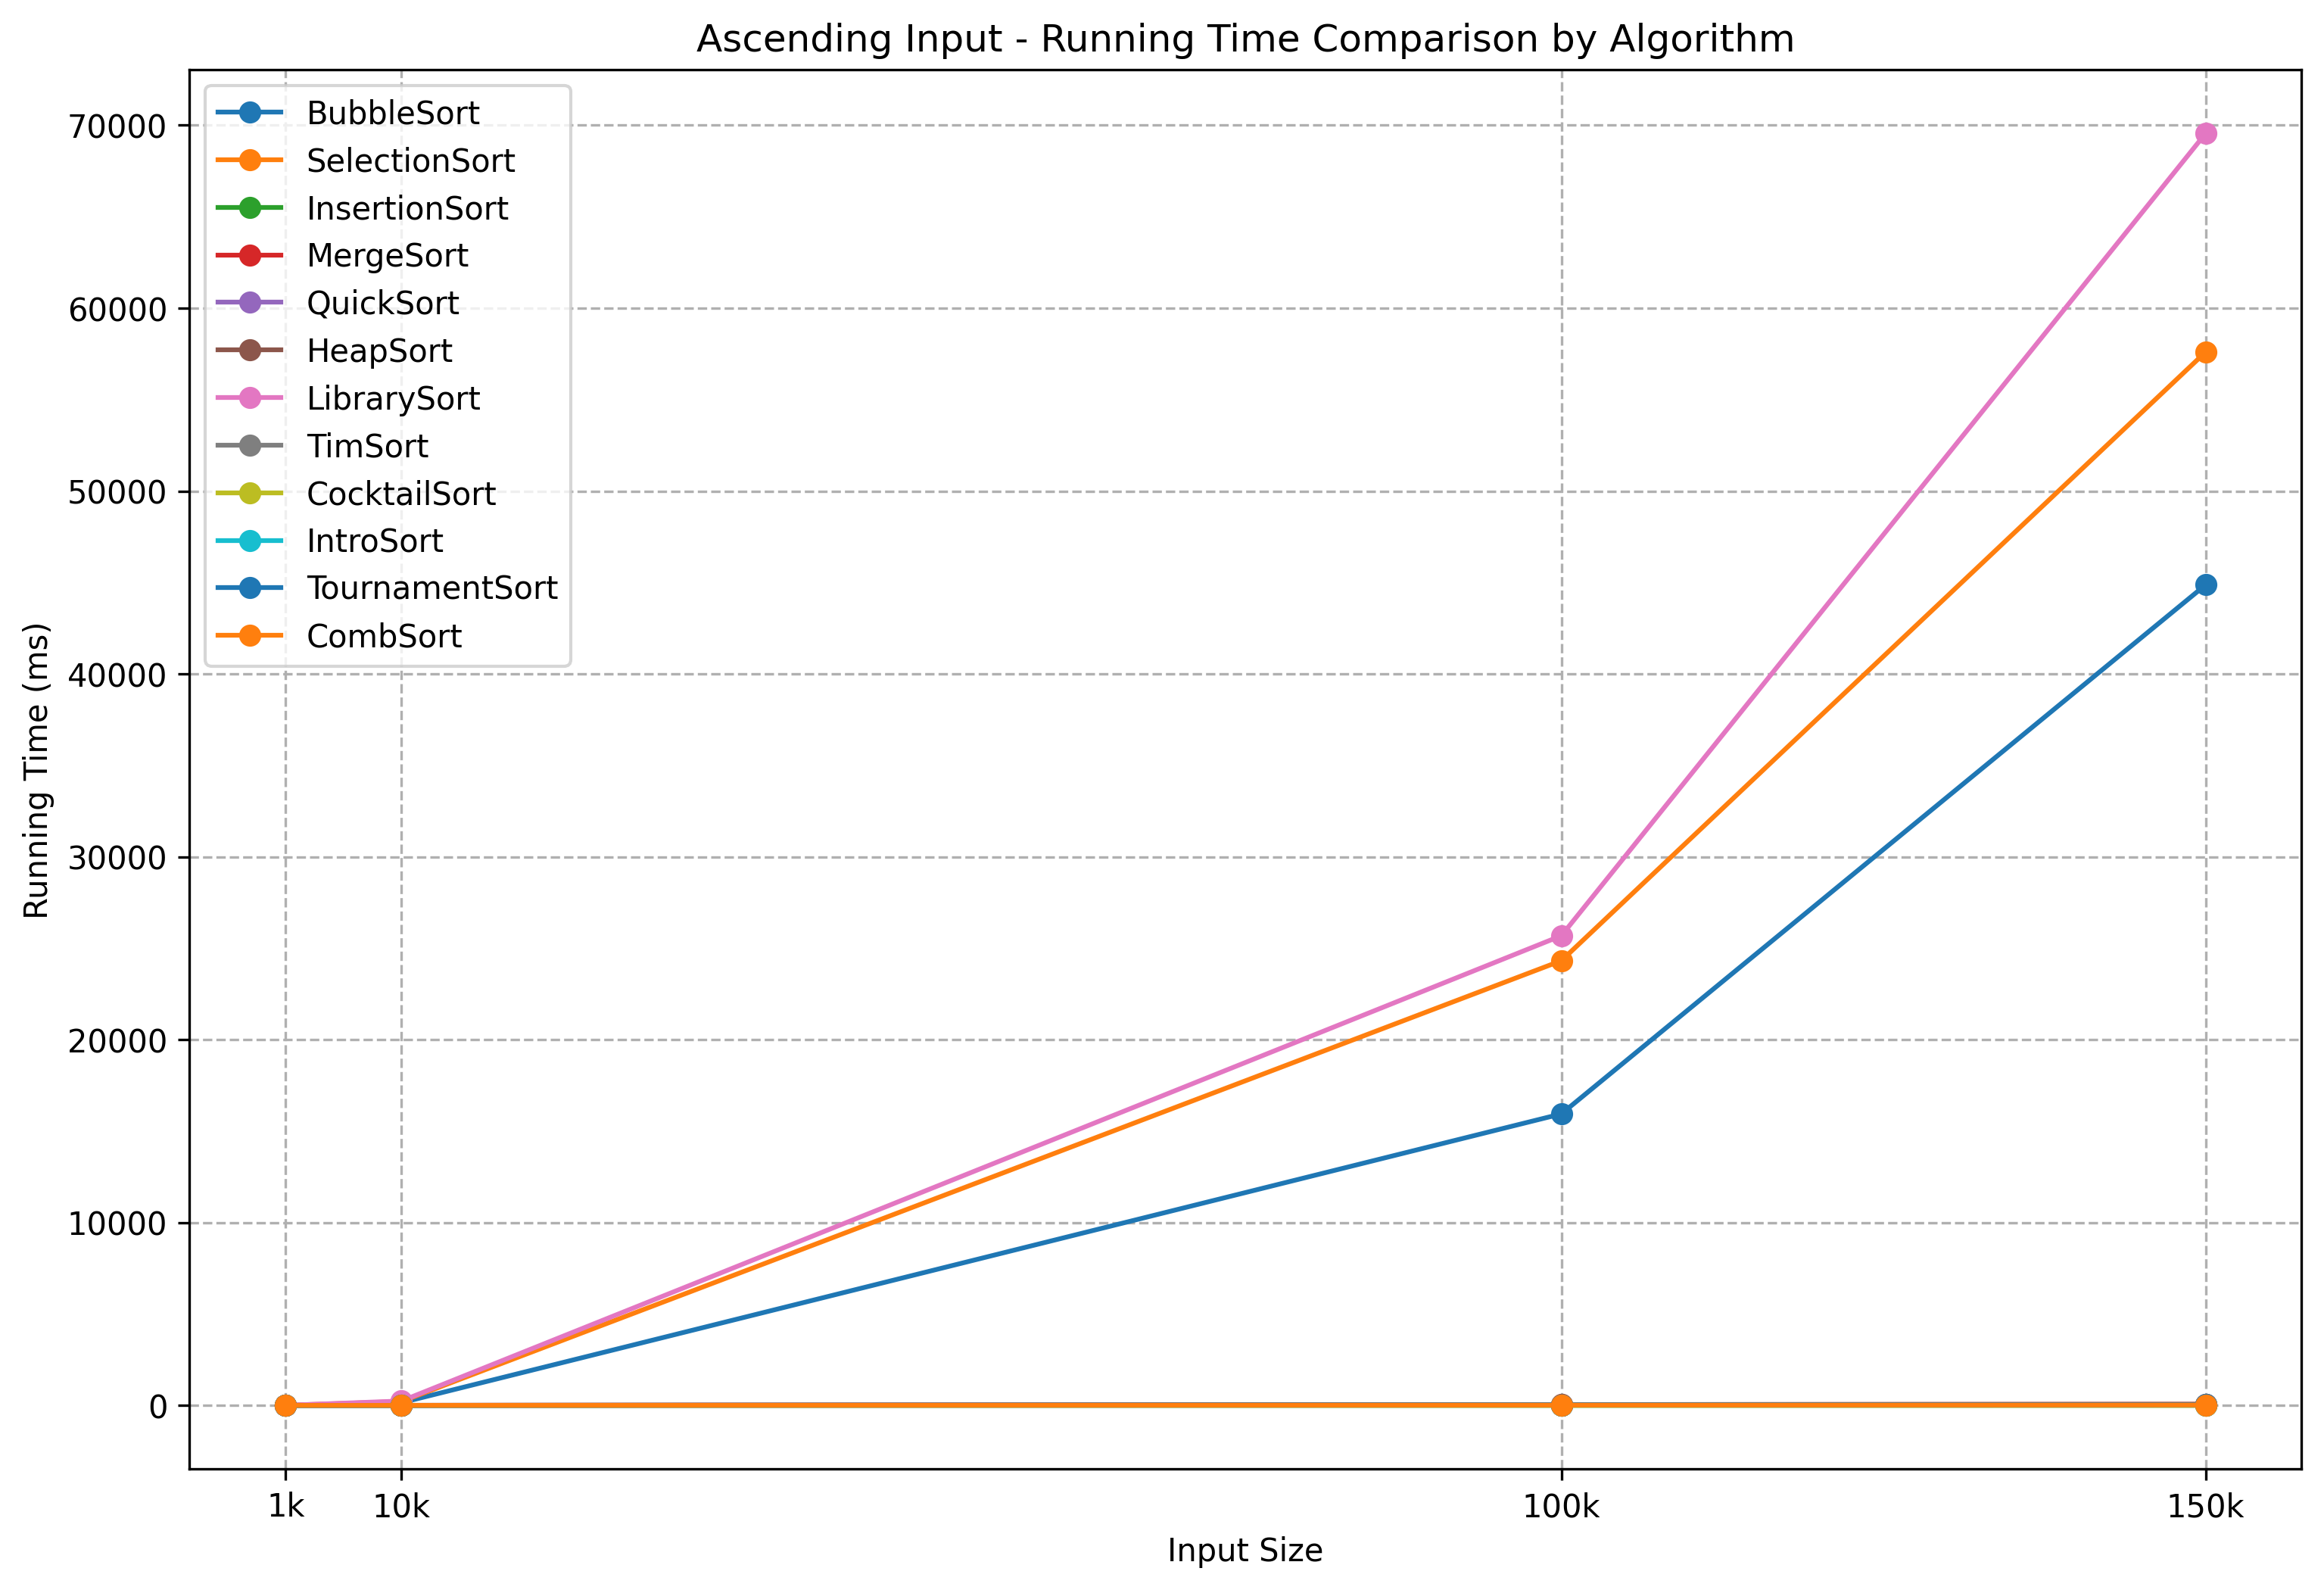
\includegraphics[width=\textwidth]{ascending.png}
    \caption{Performance on ascending (already sorted) arrays}
    \label{fig:ascending}
  \end{minipage}
  \hfill
  \begin{minipage}{0.48\textwidth}
    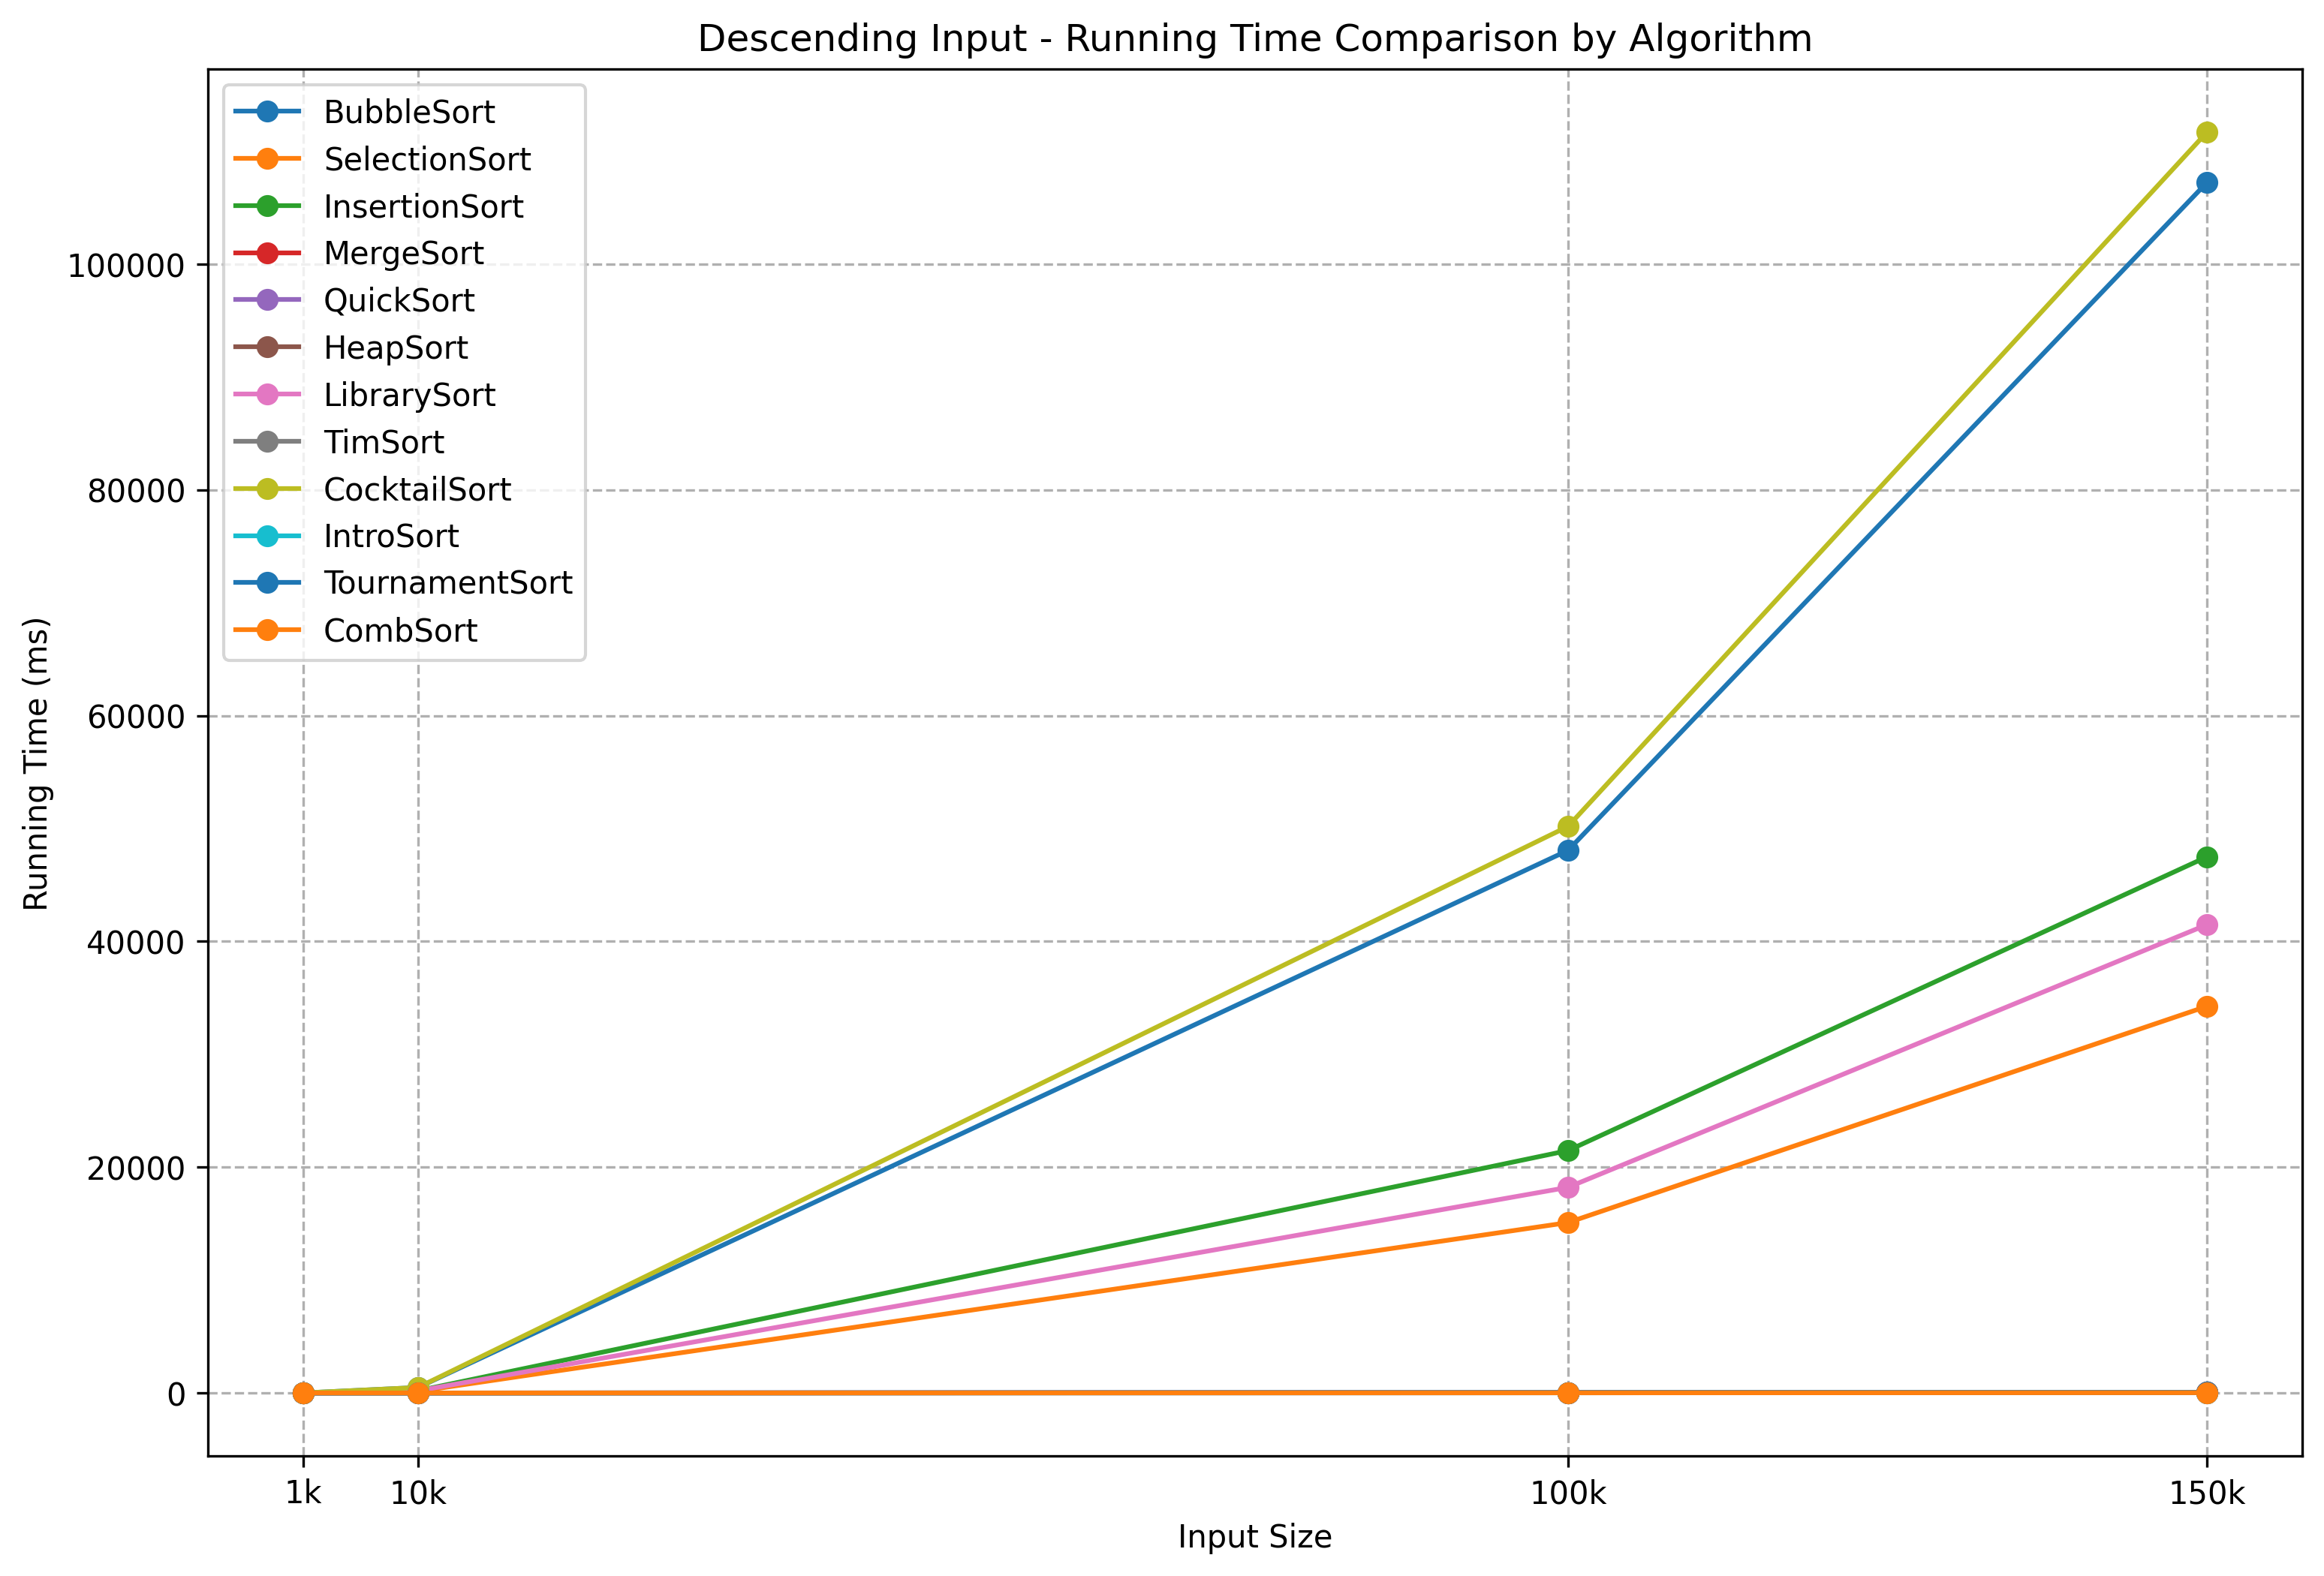
\includegraphics[width=\textwidth]{descending.png}
    \caption{Performance on descending (reverse sorted) arrays}
    \label{fig:descending}
  \end{minipage}
\end{figure*}

For sorted arrays (Figure \ref{fig:ascending}), contrary to theoretical expectations, our experimental results showed that Bubble Sort, Insertion Sort, and Library Sort performed the worst. This is particularly surprising for Insertion Sort, which theoretically should achieve O(n) time complexity on already sorted data. This discrepancy likely stems from implementation details or testing methodology issues in our code.

Reverse sorted arrays (Figure \ref{fig:descending}) presented significant challenges for several algorithms in our implementation. Cocktail Sort showed the poorest performance, followed by Bubble Sort, Insertion Sort, Library Sort, and Selection Sort. The remaining algorithms maintained relatively good performance. The poor performance of Insertion Sort on reverse sorted arrays aligns with theoretical expectations, as this represents its worst-case scenario.

\begin{figure}[h]
  \centering
  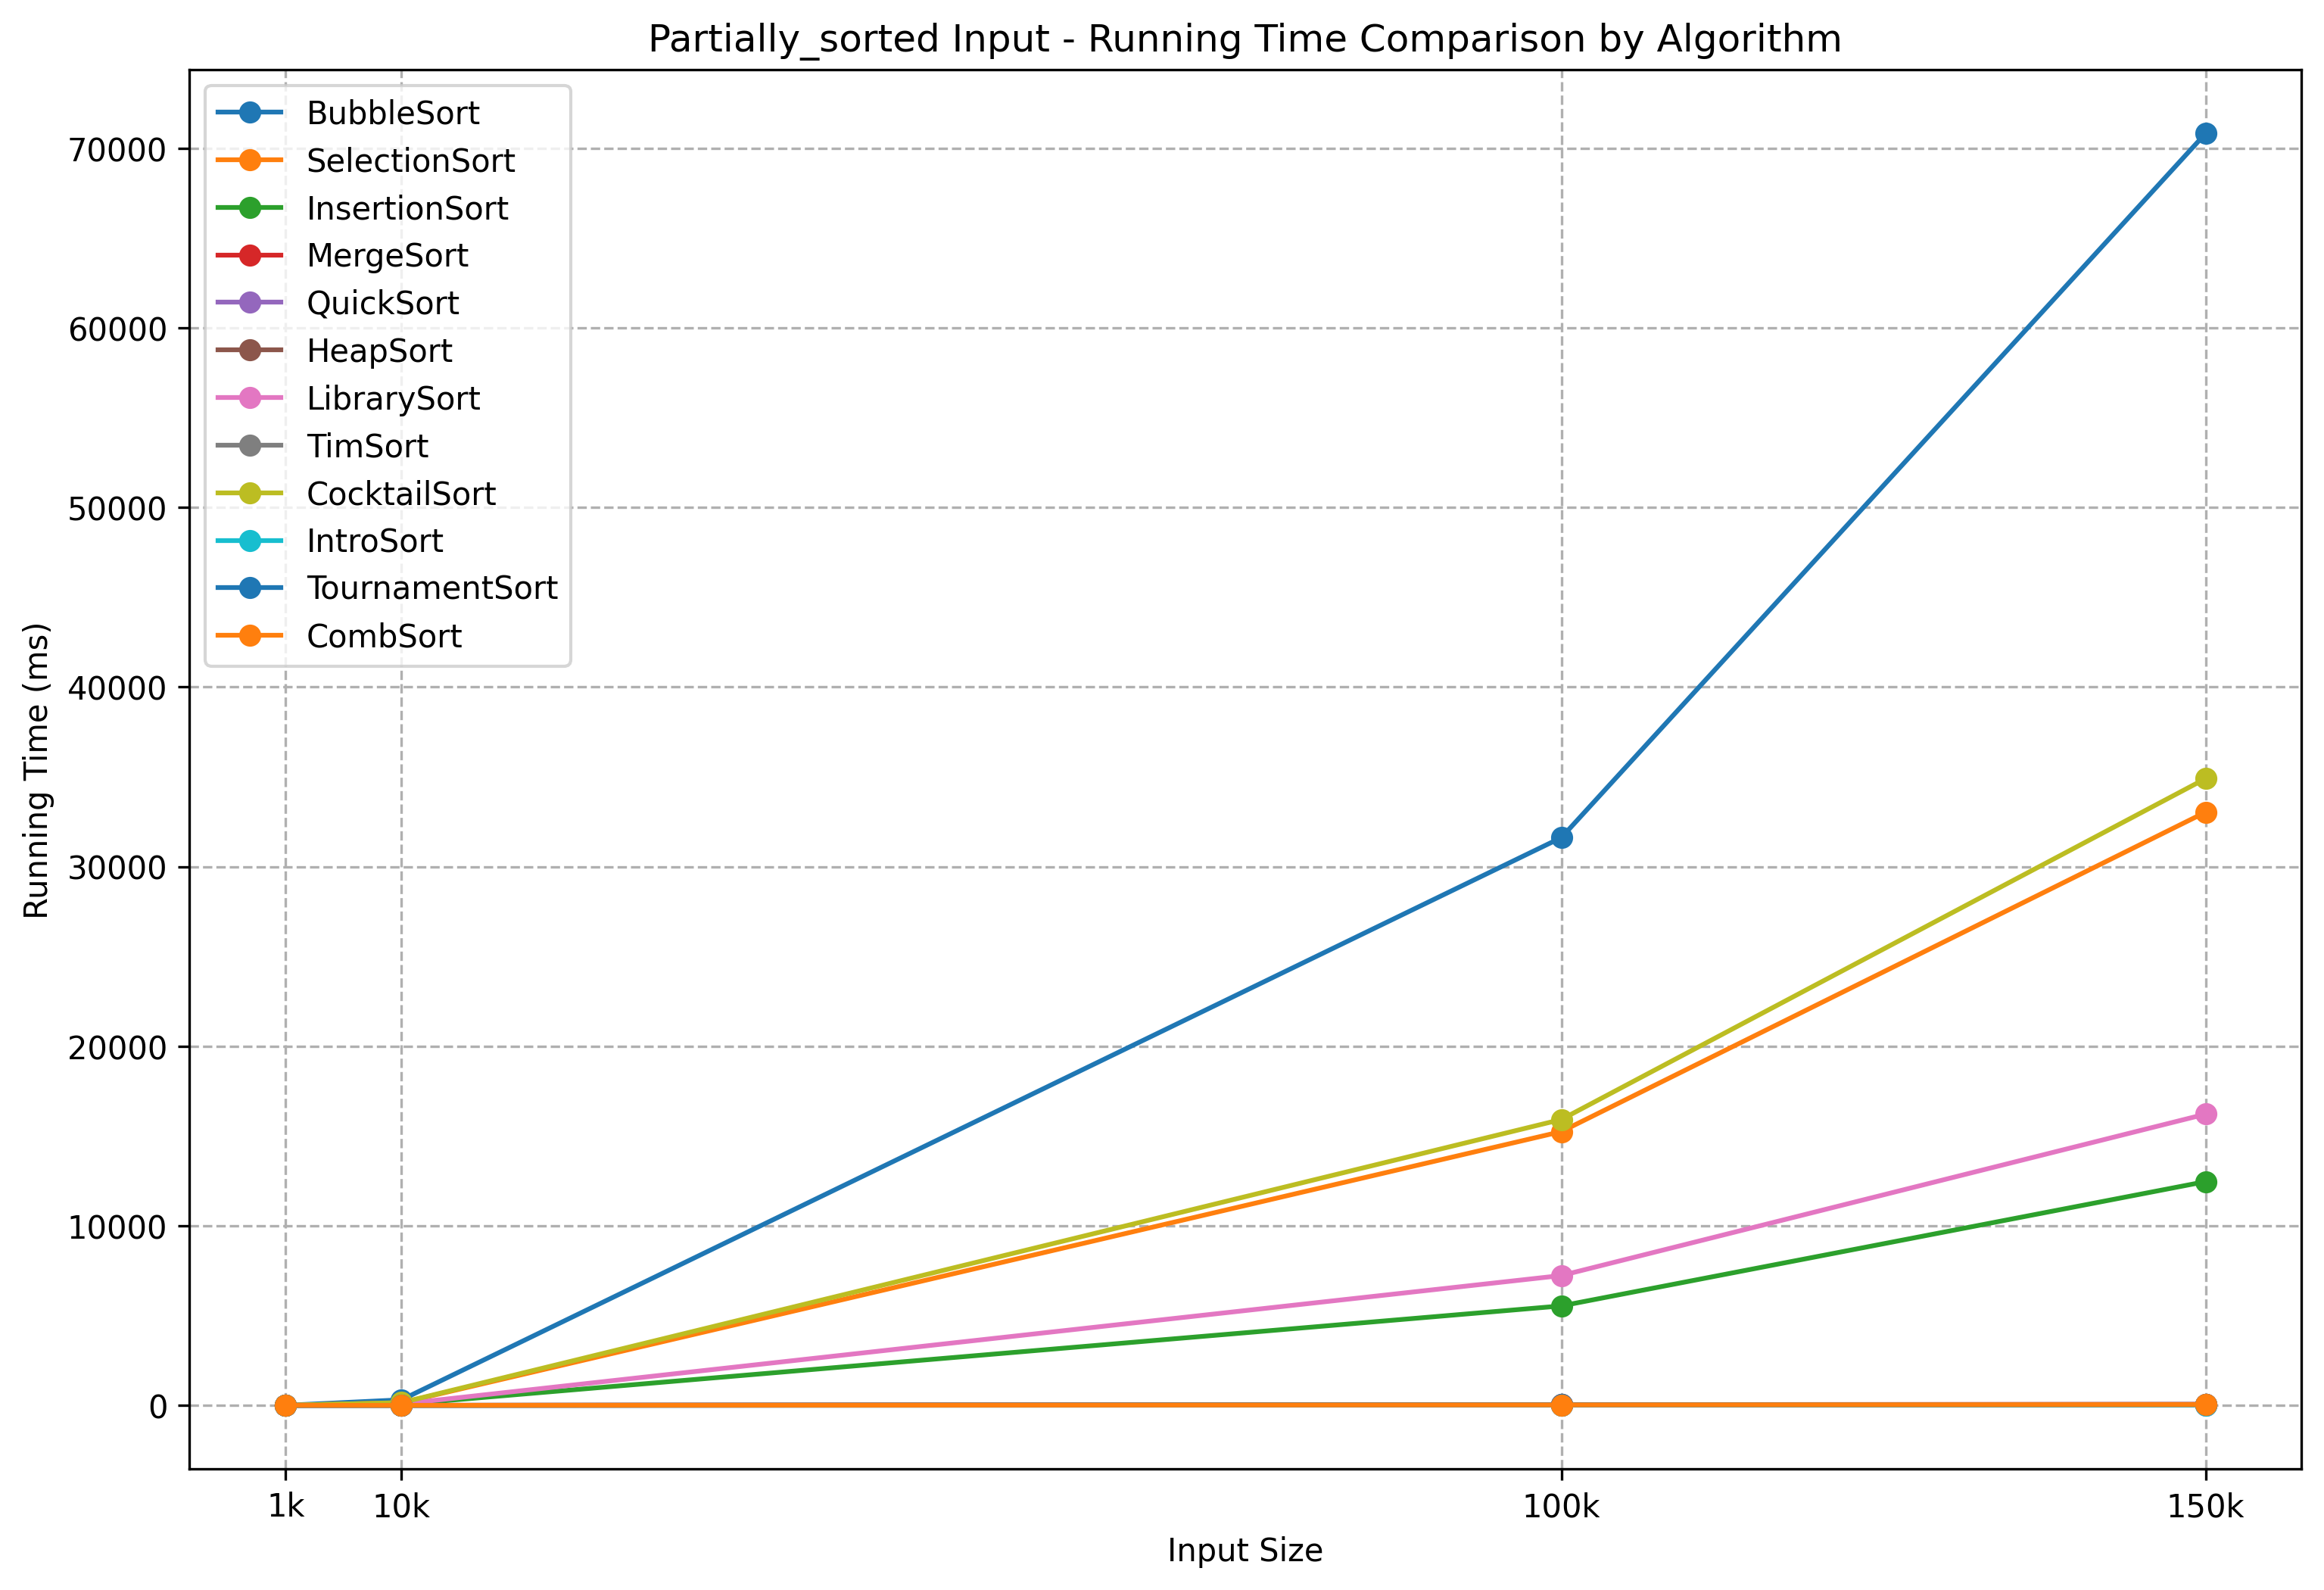
\includegraphics[width=\columnwidth]{partially_sorted.png}
  \caption{Performance on partially sorted arrays}
  \label{fig:partially}
\end{figure}

For partially sorted arrays (Figure \ref{fig:partially}), Bubble Sort performed worst, followed by Selection Sort, Cocktail Sort, Library Sort, and Insertion Sort. This is somewhat unexpected for Insertion Sort and Library Sort, which should theoretically handle partially sorted data efficiently. The more advanced algorithms (Merge Sort, Heap Sort, Quick Sort, Tim Sort, and Introsort) consistently delivered good performance across this input type.

For random arrays (Figure \ref{fig:scaling}), as expected, the quadratic algorithms showed poor scaling, with Bubble Sort performing worst, followed by Cocktail Sort, Selection Sort, and Insertion Sort.

Throughout our testing, the O(n log n) algorithms consistently outperformed the O(n²) algorithms for larger input sizes, which aligns with theoretical expectations. However, some specific behaviors, particularly the poor performance of certain algorithms on input types where they should theoretically excel, suggest potential issues in our implementation or measurement methodology. Different compiler optimizations, cache effects, or subtle implementation details might also contribute to these discrepancies.

Where our results diverge from theoretical expectations, we believe optimization opportunities exist in our code. Future work could focus on refining the implementation of these algorithms to better match their theoretical efficiency.

\subsection{Memory Usage Analysis}
We performed a theoretical analysis of the memory requirements of each algorithm based on their space complexity:

\begin{itemize}
  \item \textbf{Constant space ($O(1)$)}: Bubble Sort, Selection Sort, Insertion Sort, Heap Sort, Cocktail Sort, and Comb Sort all operate in-place, requiring only a few variables regardless of input size.
  
  \item \textbf{Logarithmic space ($O(\log n)$)}: Quick Sort and Introsort require stack space for recursion. With careful implementations, this can be bounded to logarithmic space.
  
  \item \textbf{Linear space ($O(n)$)}: Merge Sort, Tournament Sort, and Library Sort require additional memory proportional to the input size. Tim Sort also requires linear extra space in the worst case, though it attempts to minimize memory usage through various optimizations.
\end{itemize}

While we did not conduct explicit measurements of memory consumption during our experiments, the theoretical space complexity provides important guidance for algorithm selection in memory-constrained environments. The in-place algorithms (those with $O(1)$ space complexity) would theoretically be preferable when memory resources are limited, with Heap Sort being particularly attractive due to its combination of $O(n \log n)$ time complexity and constant space requirements.

\subsection{Stability Analysis}
We conducted a theoretical analysis of the stability characteristic of each algorithm. Unlike our performance and memory usage tests, this analysis was not based on empirical measurements but rather on the theoretical properties of the algorithms as described in literature.

In our theoretical analysis, the following algorithms are classified as stable:
\begin{itemize}
    \item Merge Sort
    \item Insertion Sort
    \item Bubble Sort
    \item Cocktail Shaker Sort
    \item Tim Sort
    \item Library Sort
\end{itemize}

While the following algorithms are classified as non-stable:
\begin{itemize}
    \item Quick Sort
    \item Heap Sort
    \item Selection Sort
    \item Comb Sort
    \item Tournament Sort
    \item Introsort
\end{itemize}

This stability characteristic is crucial for applications where the relative order of equal elements must be preserved, such as multi-key sorting or when maintaining database consistency across multiple sorts. Although we did not empirically verify the stability of our implementations, the theoretical classification provides important insights into algorithm selection for stability-sensitive applications.

\subsection{Overall Evaluation}
Based on our comprehensive analysis, we can make the following recommendations:

\begin{enumerate}
    \item For general-purpose sorting where performance is critical: \textbf{Introsort} provides the best balance of worst-case guarantees and practical efficiency.
    
    \item For nearly sorted data: \textbf{Tim Sort} consistently outperforms other algorithms, with \textbf{Insertion Sort} being competitive for small to moderate-sized inputs.
    
    \item For memory-constrained environments: \textbf{Heap Sort} offers guaranteed $O(n \log n)$ performance with minimal memory overhead.
    
    \item For small datasets (n < 50): \textbf{Insertion Sort} is often the most efficient choice.
    
    \item When stability is required: \textbf{Tim Sort} offers the best performance among stable algorithms, with \textbf{Merge Sort} as a good alternative.
\end{enumerate}

The traditional $O(n^2)$ algorithms (Bubble, Selection, Insertion) still have educational value and can be practical for very small inputs, but should generally be avoided for production use with large datasets.

Among the contemporary algorithms, Tim Sort and Introsort stand out for their practical efficiency and robustness across different input distributions, explaining their widespread adoption in standard libraries.

% Include all references
\nocite{*}

\bibliographystyle{ACM-Reference-Format}
\bibliography{reference}

\end{document}
